\chapter{考察}
\section{低温域の熱膨張について}
\label{sec:he_100k}
Moment法の熱膨張の結果は低温域で現実的ではない値を見積もっている.
原因を$y_0$の関数から考える.まず式(\ref{eq:moment15})より$y_0$は
\begin{eqnarray}
\label{eq:y01}
y_0= \sqrt{\frac{2\gamma\theta^2}{3k^3}A}
\end{eqnarray}
であり,$\theta=k_{\rm{B}}T$を代入し,
\begin{eqnarray}
\label{eq:y02}
y_0= \sqrt{\frac{2\gamma(k_{\rm{B}}T)^2}{3k^3}A}
\end{eqnarray}
と書ける.これを変形すると$y_0$は
\begin{eqnarray}
\label{eq:y02}
y_0= \sqrt{\frac{2\gamma}{3k^3}}k_{\rm{B}}\times \sqrt{A} \times T
\end{eqnarray}
このように書くことができる.
$\sqrt{\frac{2\gamma}{3k^3}}k_{\rm{B}}$は$k$,$\gamma$の関数であり原子間距離によって値が定まる.Cuのペアポテンシャルの$k$, $\gamma$による,最近接原子間距離と$\sqrt{\frac{2\gamma}{3k^3}}k_{\rm{B}}$の関係を図\ref{fig:y0_heat}(\subref{y0_heat1})に示す.
また,$\sqrt{A}$は$k$, $\gamma$, $T$の関数であり,簡単な2次元のグラフでは表すことができない.
しかし,実際の熱膨張の計算結果に用いられた$\sqrt{A}$の数値を見れば取り得る値の範囲がわかり傾向を掴むことができる.
それを図\ref{fig:y0_heat}(\subref{y0_heat2})に示す.
(\subref{y0_heat1})より$\sqrt{\frac{2\gamma}{3k^3}}k_{\rm{B}}$は原子間距離に対して緩やかなカーブを描きながら増加しており,低温域の急激な熱膨張には影響していないことがわかる.
また,(\subref{y0_heat1})からは,$\sqrt{A}$は,1Kから50Kにかけて急激に減少しており,逆に低温域での熱膨張を抑えていることがわかる.最後に$y_0$の残りの成分である$T$に着目すると,単純に1Kから100Kの温度変化で$y_0$を100倍していることになり,これは明らかに低温域の急激な熱膨張の原因だとわかる.これらの結果からMoment法の低温域での急激な熱膨張は,$y_0$に含まれる$T$が原因であり,$T$の増加率,実際の計算結果から考えると100K以下の結果は参考にならないと言える.
\begin{figure}[htbp]
 \begin{minipage}[b]{0.5\linewidth}
  \centering
  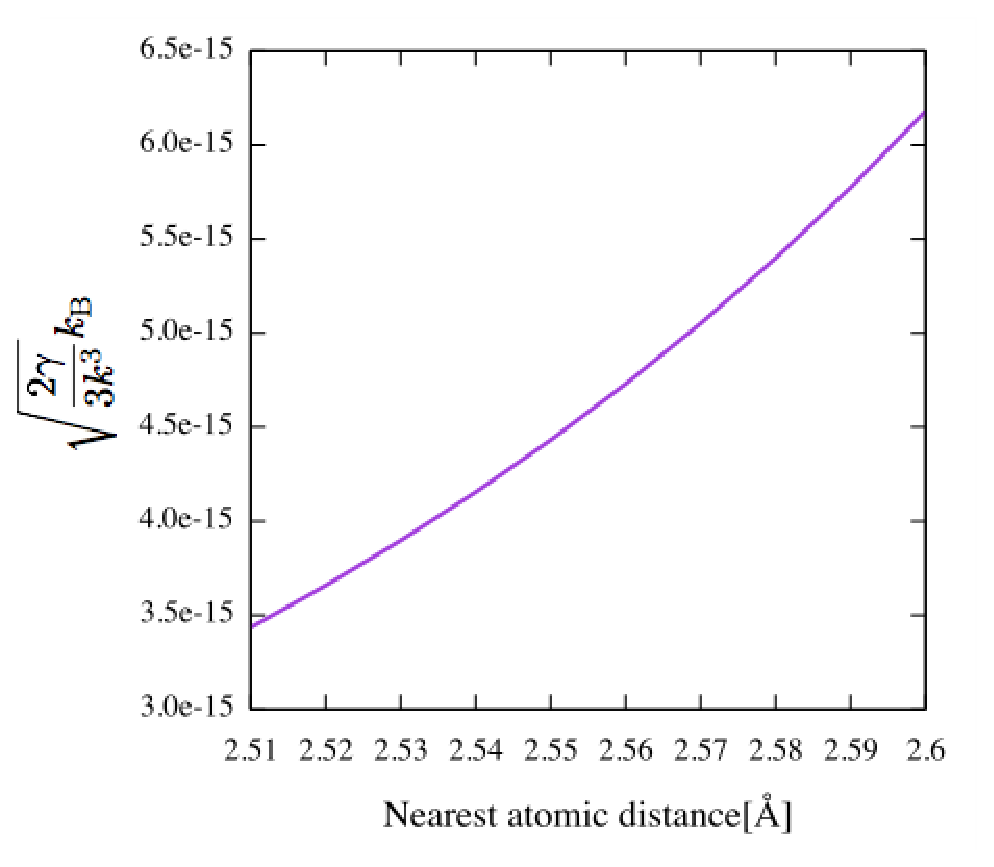
\includegraphics[keepaspectratio, scale=0.42]
  {../image/y0_no_largea_label.eps}
  \subcaption{}\label{y0_heat1}
 \end{minipage}
 \begin{minipage}[b]{0.5\linewidth}
  \centering
  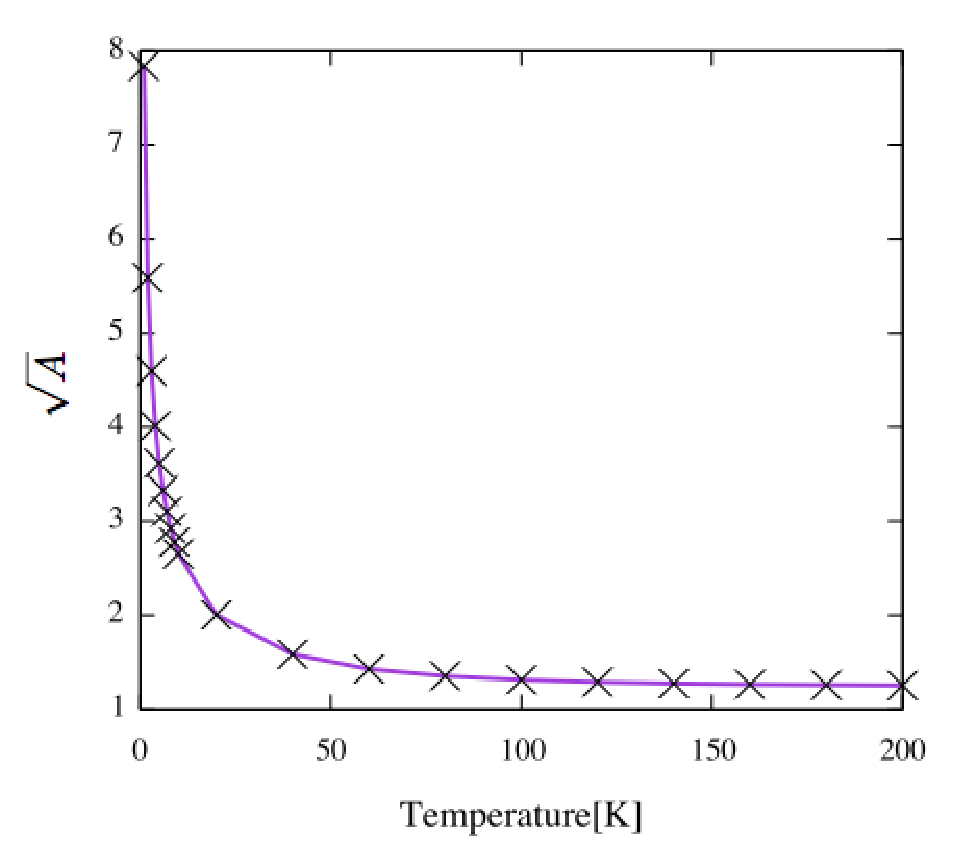
\includegraphics[keepaspectratio, scale=0.42]
  {../image/y0_largea_label.eps}
  \subcaption{}\label{y0_heat2}
 \end{minipage}
 \caption{$y_0$に含まれる関数の概形.
 (\subref{y0_heat1})は$\sqrt{\frac{2\gamma}{3k^3}}k_{\rm{B}}$は$k$,$\gamma$と原子間距離の関係,(\subref{y0_heat1})は実際の各温度での熱膨張計算で$\sqrt{A}$ が取る値を示している.$k$, $\gamma$にはCuのペアポテンシャルを用いた.
 }\label{fig:y0_heat}
\end{figure}

\section{$a_0$を変えた計算結果}
熱膨張の計算における0Kでの原子間距離に着目していく.
MomentVASPの計算は最近接原子間距離の初期値である$a_0$にVASPの構造最適化による最安定距離を使用している.それに比べMedeA, Phonopyは振動による自由エネルギーを考慮しているため0Kでの格子の長さは基底状態とは異なってくる.
例えばAlであれば0KにおけるMomentVASPの最近接原子間距離は2.856$\mathrm{\AA}$, Phonopyは2.866$\mathrm{\AA}$であり,その差は0.01$\mathrm{\AA}$ある.Moment法は$a_0$の値を変えると$k$, $\gamma$を参照する$y$の値が変わり違う結果を出してくれる.
そこで,MomentVASPの計算に使用していた$a_0$をPhonopyの0Kの原子間距離に変えることによって,結果が改善されるのではないかと考えた.
Alによる結果を図\ref{fig:a0test}に示す.

\begin{figure}[htbp]
 \begin{minipage}[b]{0.5\linewidth}
  \centering
  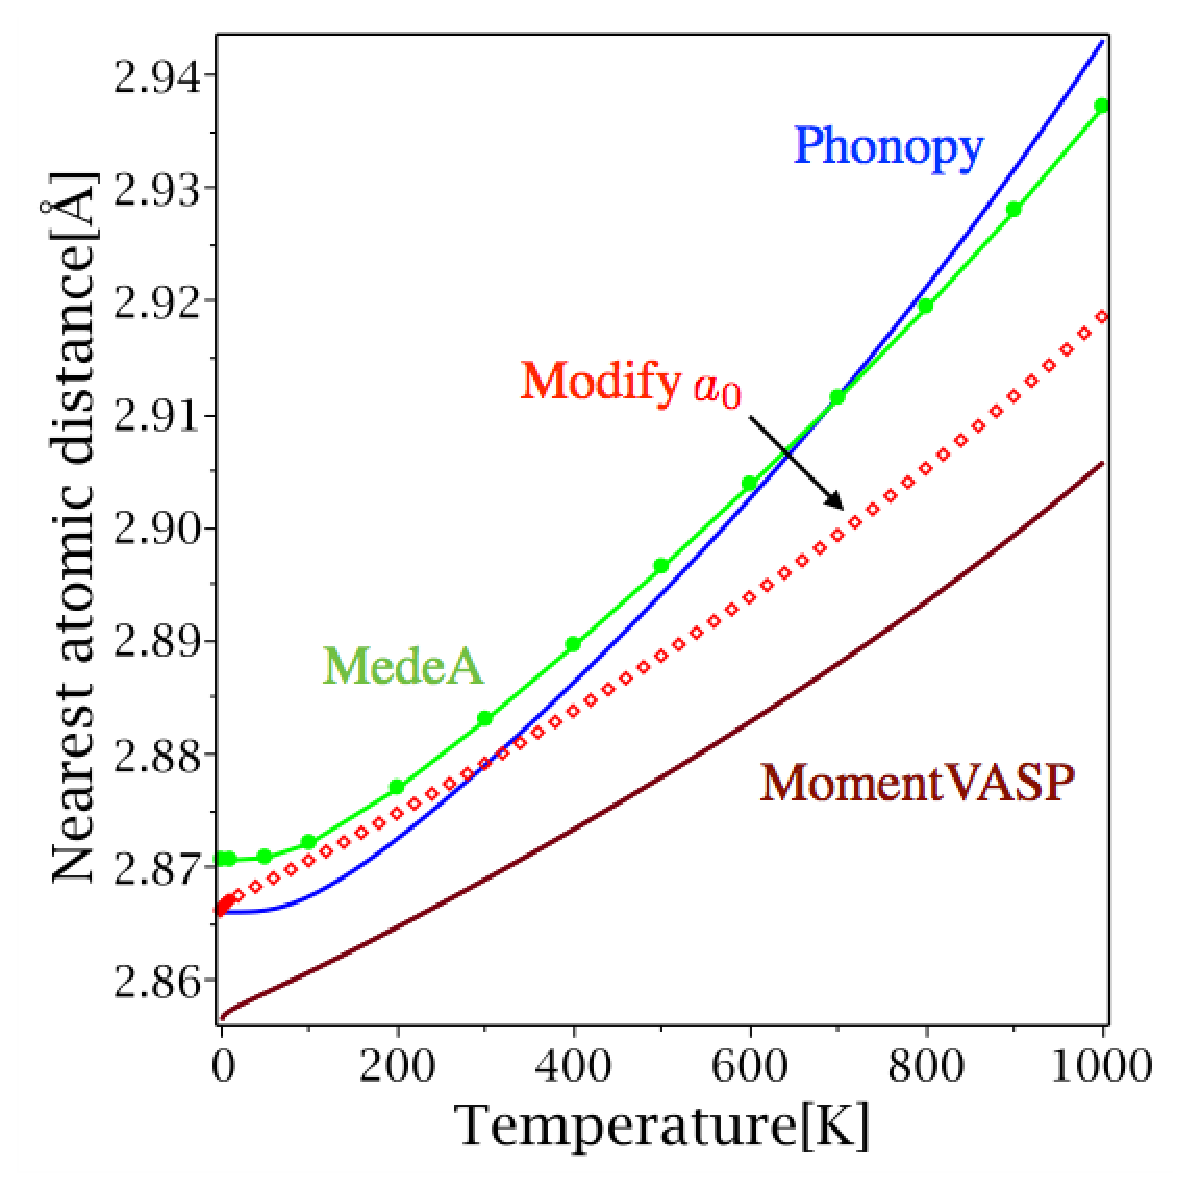
\includegraphics[keepaspectratio, scale=0.42]
  {../image_result/Al_lat_phonopy_label.eps}
  \subcaption{最近接原子間距離と温度の依存性}\label{a0test1}
 \end{minipage}
 \begin{minipage}[b]{0.5\linewidth}
  \centering
  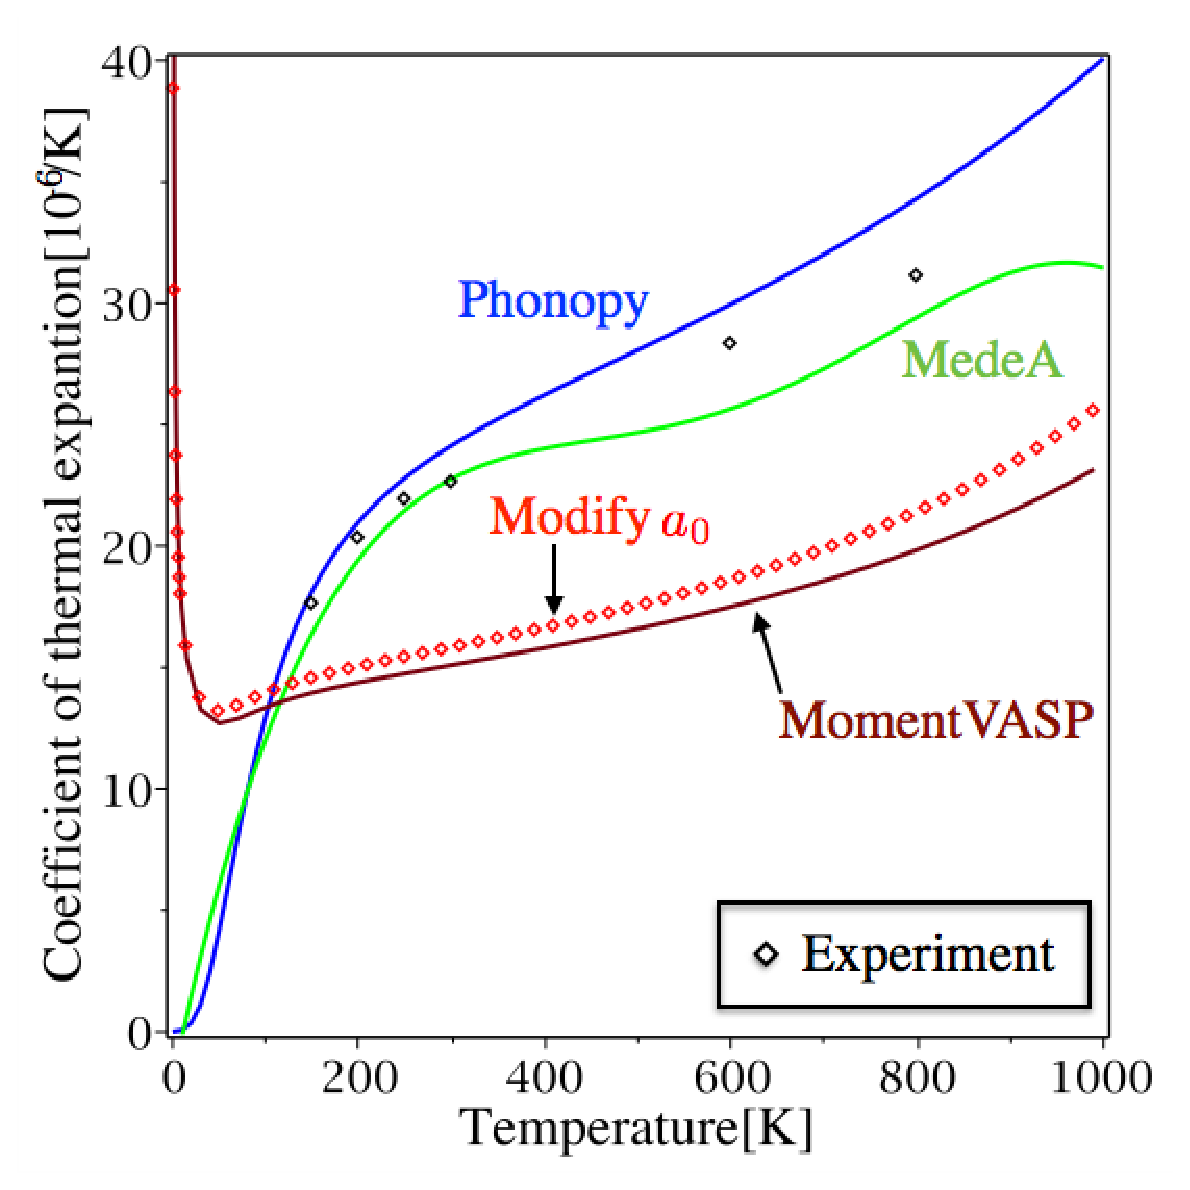
\includegraphics[keepaspectratio, scale=0.42]
  {../image_result/Al_TEcoeff_phonopy_label.eps}
  \subcaption{線膨張係数と温度の依存性.}\label{a0test2}
 \end{minipage}
 \hspace{10cm}
 \begin{minipage}[b]{0.5\linewidth}
  \centering
  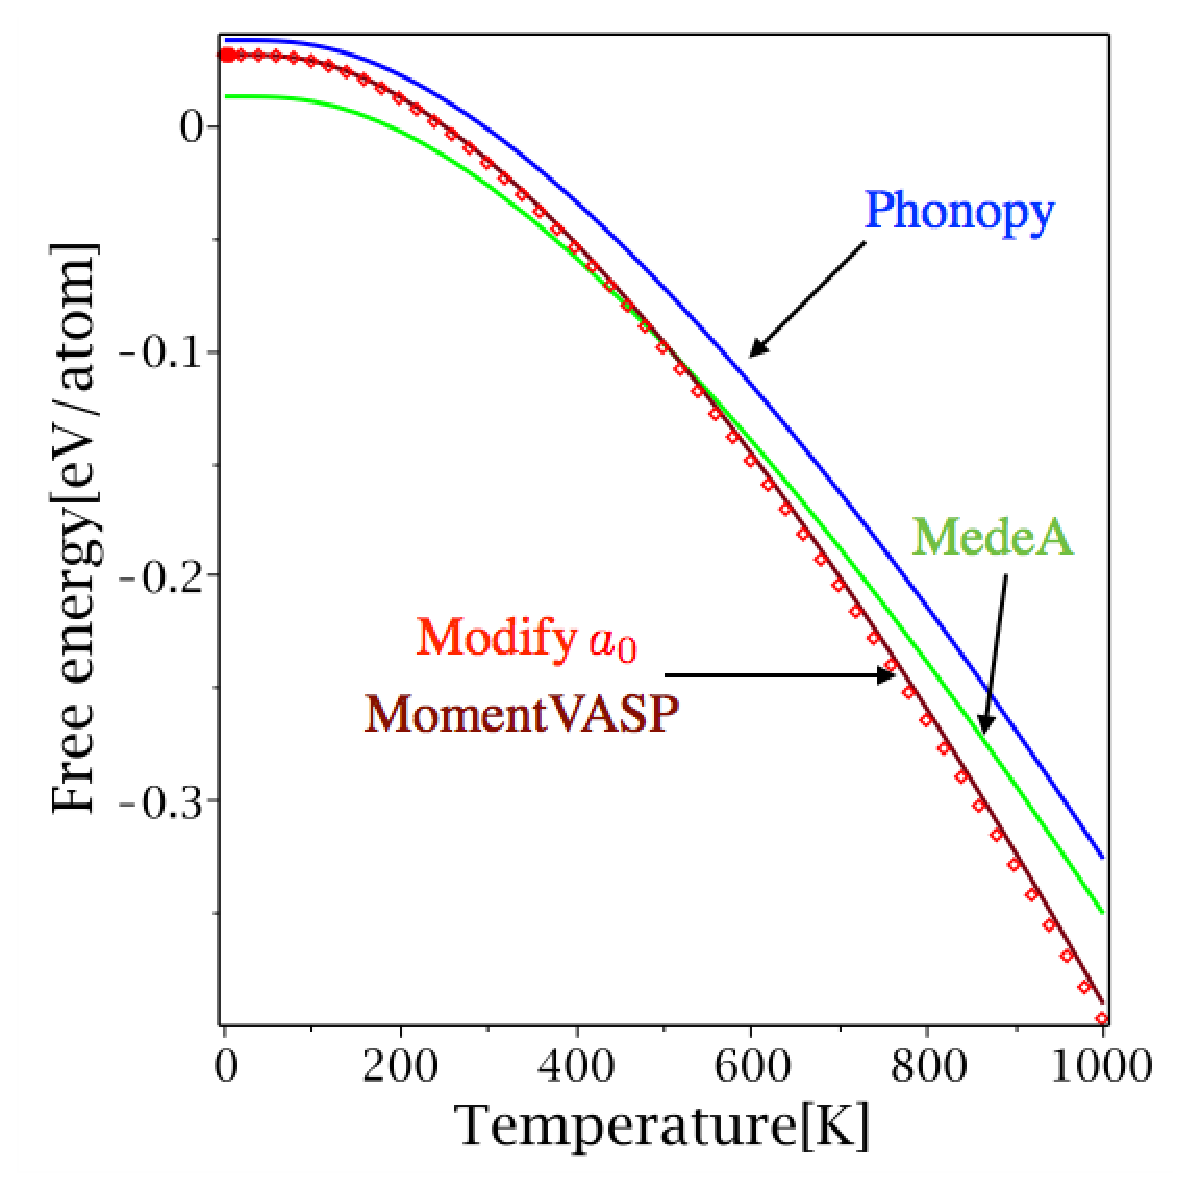
\includegraphics[keepaspectratio, scale=0.42]
  {../image_result/Al_free_phonopy_label.eps}
  \subcaption{$U_0$を含まない自由エネルギーの温度依存性.}\label{a0test3}
 \end{minipage}
 \begin{minipage}[b]{0.5\linewidth}
  \centering
  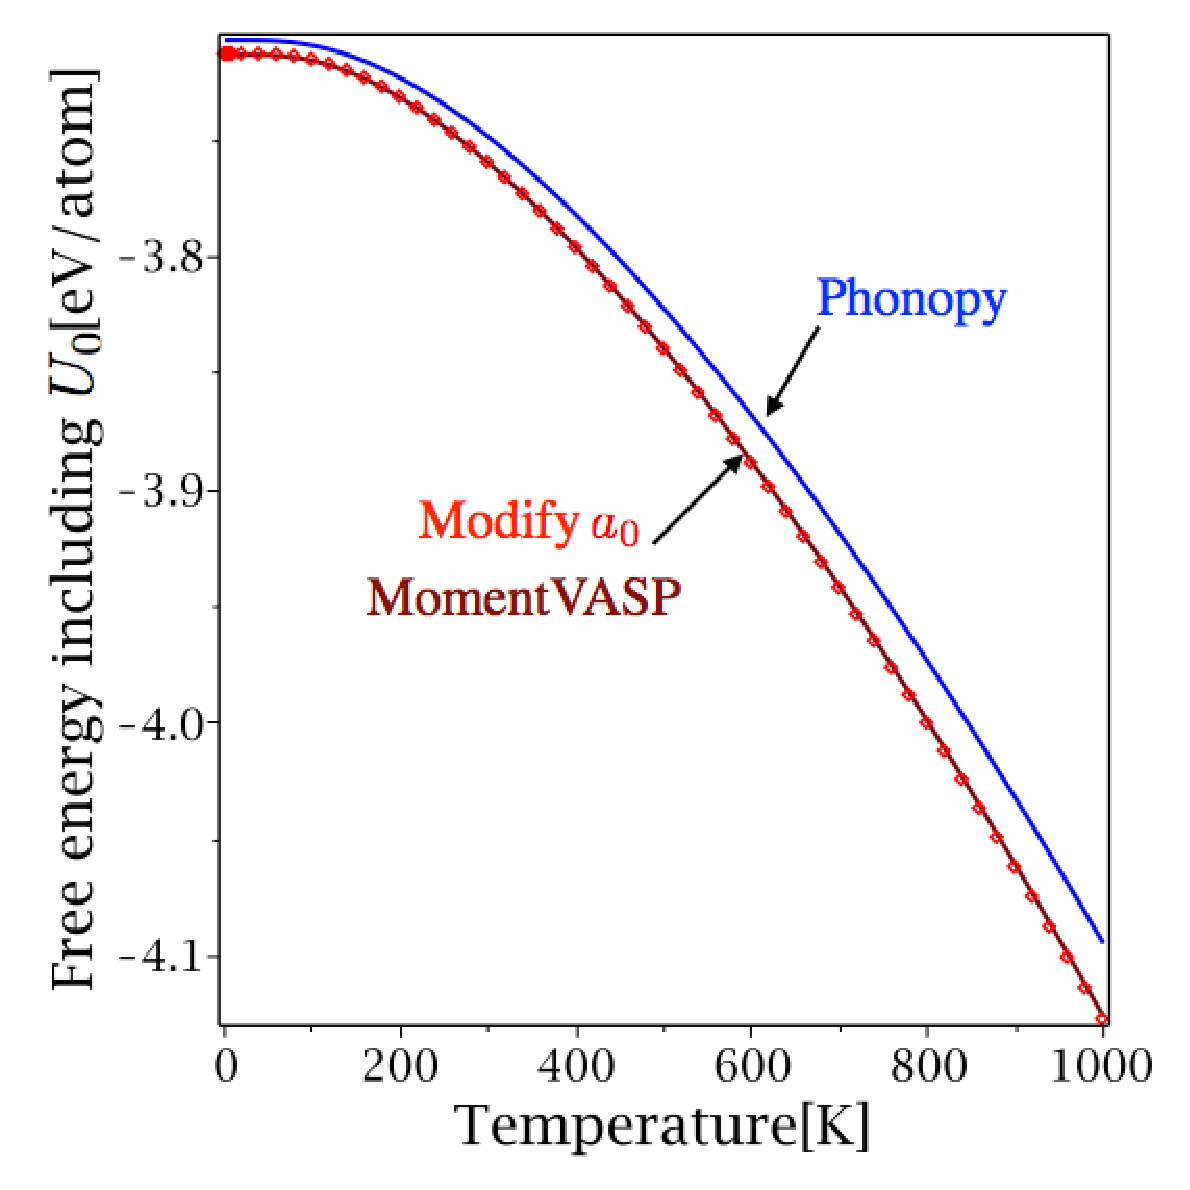
\includegraphics[keepaspectratio, scale=0.42]
  {../image_result/Al_free_u0_phonopy_label.eps}
  \subcaption{$U_0$を含んだ自由エネルギーの温度依存性.}\label{a0test4}
 \end{minipage}
 \caption{AlのMomentVASPの$a_0$をPhonopyの0Kでの最近接原子間距離に変えることによる計算結果の変化.}\label{fig:a0test}
\end{figure}

図中のラベルModify $a_0$がMomentVASPの$a_0$をPhonopyの0Kでの最近接原子間距離に変化させた計算結果である.
(\subref{a0test1})より,$a_0$をPhonopyと揃えたため0Kで同じ距離から熱膨張を開始しているが,その後の変化は元のMomentVaspとあまり変わらない結果となった.(\subref{a0test2})の線膨張係数で比較すると若干ではあるがPhonopyと実験値に近づいていることがわかる.
自由エネルギーの比較では(\subref{a0test3}),(\subref{a0test4})ともにModify $a_0$の値はPhonopyから遠ざかる方に変化している.
また,1000Kでの最近接原子間距離の差は強引ではあるが小さくなっているにも関わらず,自由エネルギーの値の差は小さくならなかった.
よって,0Kの最近節原子間距離をPhonopyと揃えるという試みは熱膨張係数のみ若干であるが改善されるという結果となった.

